% Build: tectonic --untrusted --keep-logs scheduler-work-plan.tex
% Self-contained LaTeX source. Diagrams are vector graphics drawn with TikZ.
\documentclass[10pt,letterpaper]{article}
\usepackage[margin=0.72in,headheight=15pt,headsep=18pt,footskip=24pt]{geometry}
\usepackage{fontspec}
\setmainfont{texgyreheros-regular.otf}[BoldFont=texgyreheros-bold.otf,ItalicFont=texgyreheros-italic.otf,BoldItalicFont=texgyreheros-bolditalic.otf]
\newfontfamily\displayfont{texgyrepagella-regular.otf}[BoldFont=texgyrepagella-bold.otf,ItalicFont=texgyrepagella-italic.otf]
\setmonofont{lmmono10-regular.otf}[Scale=0.95]
\usepackage[table]{xcolor}
\usepackage{array,tabularx,booktabs}
\usepackage{enumitem}
\usepackage{tikz}
\usetikzlibrary{arrows.meta,positioning,fit,backgrounds,calc}
\usepackage{amsmath}
\usepackage{fancyhdr}
\usepackage{hyperref}
\definecolor{ink}{HTML}{172C40}
\definecolor{muted}{HTML}{53687A}
\definecolor{accent}{HTML}{007E80}
\definecolor{light}{HTML}{EEF6F5}
\definecolor{rulecolor}{HTML}{CCD9DF}
\definecolor{paperblue}{HTML}{F1F5F8}
\hypersetup{colorlinks=true,linkcolor=accent,urlcolor=accent,pdftitle={Custom Job Execution System - Reviewed Work Plan},pdfauthor={Slurm-Aware project},pdfsubject={Controller, Docker workers, execution lifecycle, and a replaceable scheduling interface}}
\pagestyle{fancy}
\fancyhf{}
\fancyhead[L]{\small\color{muted}SLURM-AWARE PROJECT / EXECUTION SYSTEM}
\fancyhead[R]{\small\color{muted}WORK PLAN / v1.0}
\fancyfoot[L]{\small\color{muted}Design proposal \textbullet\ 31 October 2026}
\fancyfoot[R]{\small\color{muted}\thepage}
\renewcommand{\headrulewidth}{0.4pt}
\renewcommand{\footrulewidth}{0pt}
\setlength{\parindent}{0pt}
\setlength{\parskip}{6pt}
\setlength{\tabcolsep}{6pt}
\renewcommand{\arraystretch}{1.22}
\setlist[itemize]{leftmargin=15pt,itemsep=3pt,topsep=4pt,parsep=0pt}
\setlist[enumerate]{leftmargin=18pt,itemsep=4pt,topsep=4pt,parsep=0pt}
\emergencystretch=2em
\color{ink}
\newcolumntype{Y}{>{\raggedright\arraybackslash}X}
\newcolumntype{P}[1]{>{\raggedright\arraybackslash}p{#1}}
\newcommand{\pagetitle}[2]{\vspace*{1pt}{\small\bfseries\color{accent}#1}\par\vspace{3pt}{\displayfont\fontsize{24}{28}\selectfont #2}\par\vspace{7pt}}
\newcommand{\lead}[1]{\par\vspace{3pt}\textbf{#1}\ }
\newcommand{\packet}[2]{\par\vspace{9pt}{\large\bfseries\color{accent}#1}\hspace{6pt}{\large\bfseries #2}\par}
\newcommand{\callout}[1]{\par\vspace{5pt}\begingroup\setlength{\fboxsep}{10pt}\colorbox{light}{\parbox{\dimexpr\linewidth-20pt\relax}{#1}}\endgroup\par\vspace{5pt}}
\newcommand{\code}[1]{\texttt{#1}}
\tikzset{
  box/.style={draw=rulecolor,rounded corners=3pt,fill=white,align=center,minimum height=0.63cm,text width=3.0cm,font=\small,inner sep=6pt},
  active/.style={box,fill=light,draw=accent,thick},
  arrow/.style={-{Latex[length=2mm]},draw=muted,thick},
  flowlabel/.style={font=\scriptsize,color=muted,fill=white,inner sep=2pt,align=center},
  group/.style={draw=rulecolor,rounded corners=5pt,fill=paperblue,inner sep=12pt},
  phase/.style={box,text width=3.0cm,minimum height=0.82cm,font=\small}
}

\begin{document}

% PAGE 1
\pagetitle{PURPOSE AND SCOPE}{Build the execution system first.}
{\large A reviewed implementation plan for real jobs on Docker workers}\par
\vspace{4pt}
Build a small Slurm-free system that accepts jobs, assigns them to worker nodes,
launches real processes, and records their outcomes. Keep job selection behind a
replaceable interface so FIFO and a future RL picker use the same execution path.

\callout{\textbf{First execution demonstration (W4):} one controller and two Docker workers
execute a mixed workload, respect allocation capacity and retain logs and outcomes.
\textbf{Accepted baseline (W6):} recovery checks plus repeatable replay and complete reports.}

\lead{What this plan covers.} Job and worker contracts, durable controller state,
resource accounting, placement, process execution, networking, cancellation,
reconciliation, Docker packaging, workload replay, and evaluation reports.

\lead{Working assumptions.} One active controller; trusted Linux jobs; one worker
per job; CPU and memory scheduling; several concurrent jobs per worker when requests
fit. Python, SQLite, HTTP/JSON, and Docker Compose are proposed implementation defaults,
not previously finalized language commitments.

\lead{Scope boundary.} Training a new RL policy is a later workstream. This plan prepares
its observation/action interface. Multi-machine jobs, GPU execution, hostile multi-user
isolation, high-availability controllers, and a general-purpose cluster platform are later
extensions. Work is sequenced by acceptance gates; no calendar or staffing commitment is assumed.

\vspace{5pt}
\begin{tabularx}{\linewidth}{@{}P{1.30in}YY@{}}
\toprule
\textbf{Current asset} & \textbf{Verified repository state} & \textbf{Use in the new system} \\
\midrule
Simulator & Event-based replay, resource constraints, fixed-weight scheduling and metrics. & Reuse concepts and tested resource checks; later expose decision boundaries. \\
Workload generator & Repeatable traces; includes runtime labels and may generate multi-node jobs. & Add single-worker execution manifests and real command workloads. \\
RL code & Gaussian weight-bandit training, one action per trace. & Preserve as an offline baseline; it is not the sequential picker. \\
Docker environment & Existing image and Compose services launch Slurm. & Add a separate custom-runner image and Compose configuration. \\
Execution system & No custom controller or worker agents yet. & New work specified by this plan. \\
\bottomrule
\end{tabularx}

\lead{Baseline and status.} Repository HEAD is \code{06a6416}. Existing simulator edits
and other local files remain uncommitted and must be preserved. PyTorch is absent from
the current virtual environment; no model checkpoints were found. Those facts do not
block building the execution path. Plan review findings and their disposition appear
on page~\pageref{reviewpage}; they are design findings, not completed system tests.

\newpage
% PAGE 2
\pagetitle{ARCHITECTURE}{Keep decisions separate from execution.}
The controller owns scheduling state and assignments. Workers own local processes.
The picker sees a snapshot and returns a choice; it does not mutate resource counters
or send launch requests.

\begin{center}
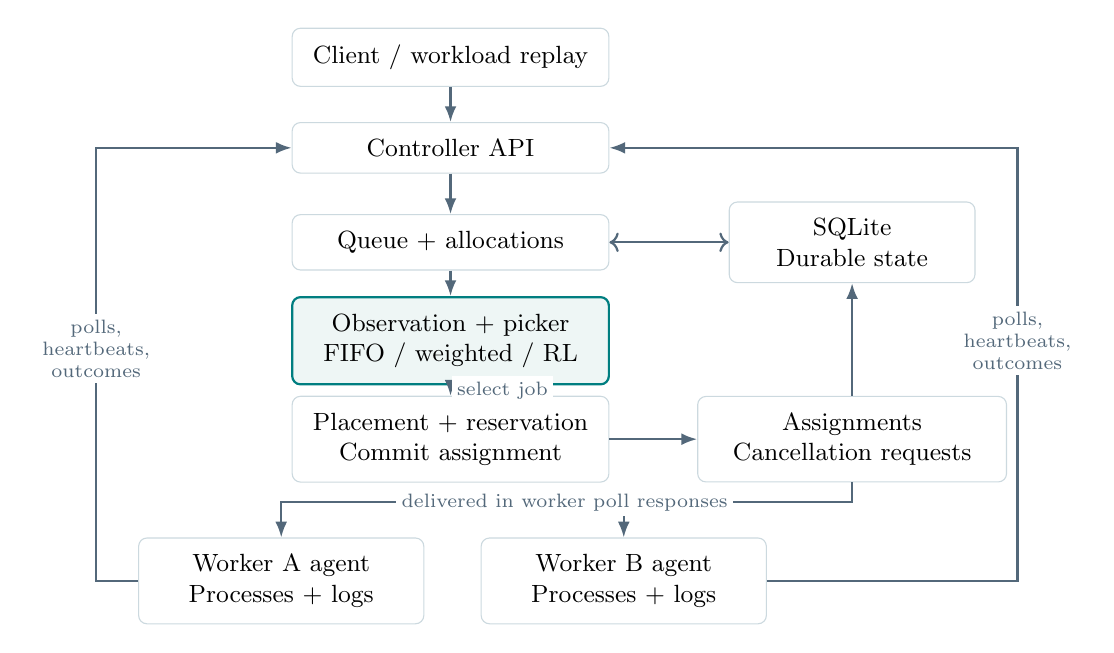
\begin{tikzpicture}
  \node[box,text width=3.6cm] (client) at (0,0) {Client / workload replay};
  \node[box,text width=3.6cm] (api) at (0,-1.15) {Controller API};
  \node[box,text width=3.6cm] (state) at (0,-2.35) {Queue + allocations};
  \node[box,text width=2.7cm] (db) at (5.1,-2.35) {SQLite\\Durable state};
  \node[active,text width=3.6cm] (picker) at (0,-3.6) {Observation + picker\\FIFO / weighted / RL};
  \node[box,text width=3.6cm] (commit) at (0,-4.85) {Placement + reservation\\Commit assignment};
  \node[box,text width=3.5cm] (outbox) at (5.1,-4.85) {Assignments\\Cancellation requests};
  \node[box,text width=3.2cm] (wa) at (-2.15,-6.65) {Worker A agent\\Processes + logs};
  \node[box,text width=3.2cm] (wb) at (2.2,-6.65) {Worker B agent\\Processes + logs};
  \draw[arrow] (client) -- (api);
  \draw[arrow] (api) -- (state);
  \draw[arrow,<->] (state) -- (db);
  \draw[arrow] (state) -- (picker);
  \draw[arrow] (picker) -- node[flowlabel,right]{select job} (commit);
  \draw[arrow] (commit) -- (outbox);
  \draw[arrow] (outbox) -- (db);
  \draw[arrow] (outbox.south) -- (5.1,-5.65) -- (-2.15,-5.65) -- (wa.north);
  \draw[arrow] (2.2,-5.65) -- (wb.north);
  \node[flowlabel] at (1.45,-5.65) {delivered in worker poll responses};
  \draw[arrow] (wa.west) -- (-4.5,-6.65) -- (-4.5,-1.15) -- (api.west);
  \node[flowlabel,text width=1.6cm] at (-4.5,-3.7) {polls,\ heartbeats,\ outcomes};
  \draw[arrow] (wb.east) -- (7.2,-6.65) -- (7.2,-1.15) -- (api.east);
  \node[flowlabel,text width=1.6cm] at (7.2,-3.6) {polls,\ heartbeats,\ outcomes};
\end{tikzpicture}
\end{center}

\lead{Central scheduling, worker pull.} Workers register and poll with their session
identity, active attempts, and unacknowledged events. The controller returns assignments
already committed to that worker. A worker never independently removes the next job
from the shared queue. Polling order must not become an accidental scheduling policy.

\lead{One decision boundary.} On an arrival, outcome, worker-state change, or timer,
build a snapshot containing all queued jobs and feasibility information. The picker
returns \code{SelectJob(id)} or \code{Wait}. Revalidate the snapshot, choose a compatible
worker deterministically, and commit the reservation before delivery. Waiting schedules
a positive-time wakeup, including when no processes are running.

\lead{Docker's role.} Compose supplies node containers and networking. Our controller
assigns jobs. Each worker launches child processes inside its container; nested Docker
and access to the host Docker socket are unnecessary for this prototype. Container
limits constrain aggregate worker usage. Declared per-job allocations alone do not
enforce individual process CPU or memory limits.

\newpage
% PAGE 3
\pagetitle{CONTRACTS AND STATE}{Make uncertainty part of the model.}
Separate the submitted job from an execution attempt. A new attempt is an explicit
retry; repeated delivery of the same attempt is not permission to launch another process.

\begin{tabularx}{\linewidth}{@{}P{1.14in}Y@{}}
\toprule
\textbf{Contract} & \textbf{Minimum contents} \\
\midrule
JobSpec & Job ID and submission key; argument list; working directory; environment; CPU/memory request; execution timeout; optional duration estimate and input reference. Actual runtime is an outcome. \\
WorkerSession & Stable worker ID, current reporting session, execution-session identity, capacity, health and active attempt inventory. New registration does not erase unresolved commitments. \\
Attempt & Attempt ID, job ID, worker/session, state, reserved resources, cancellation request, start/finish evidence, exit status and output references. \\
Event & Stable event ID, attempt/session identity, event type, timestamps and payload. Worker retains events until acknowledged. \\
Observation & Snapshot version; all queued requests and ages; worker availability after commitments; in-flight/running attempts; feasible choices; timer/control-rule state. No future arrivals or true remaining runtimes. \\
\bottomrule
\end{tabularx}

\vspace{7pt}
\begin{center}
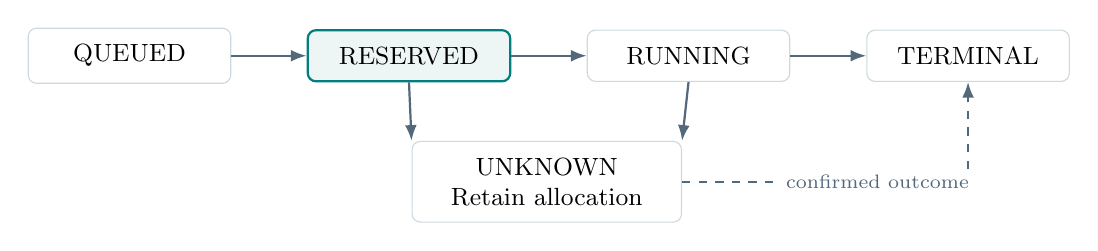
\begin{tikzpicture}[box/.append style={text width=2.15cm,minimum height=0.65cm,font=\small}]
  \node[box] (q) at (0,0) {QUEUED};
  \node[active,text width=2.15cm] (r) at (3.55,0) {RESERVED};
  \node[box] (run) at (7.1,0) {RUNNING};
  \node[box] (term) at (10.65,0) {TERMINAL};
  \node[box,text width=3.0cm] (unknown) at (5.3,-1.6) {UNKNOWN\\Retain allocation};
  \draw[arrow] (q) -- (r);
  \draw[arrow] (r) -- (run);
  \draw[arrow] (run) -- (term);
  \draw[arrow] (r.south) -- (unknown.north west);
  \draw[arrow] (run.south) -- (unknown.north east);
  \draw[arrow,dashed] (unknown.east) -- (10.65,-1.6) -- (term.south);
  \node[flowlabel] at (9.5,-1.6) {confirmed outcome};
\end{tikzpicture}
\end{center}
{\small\color{muted}Terminal outcomes: success, failure, timeout, cancellation, or LOST after
confirmed environment destruction without an exit result. UNKNOWN may reconcile to RUNNING.}

\lead{Four invariants govern every transition.}
\begin{enumerate}
\item Reserve resources and record an attempt in one controller transaction before delivery.
Capacity includes both reserved and running allocations.
\item Keep one unresolved attempt per job. Missing heartbeats make a worker unavailable;
they do not prove that its processes stopped.
\item Release capacity once, after the managed process group is stopped or execution-environment
loss is confirmed. Cancellation remains requested until termination is confirmed.
\item Deduplicate by identity. A current reporting session may reconcile older execution
attempts, but cannot let stale messages overwrite newer attempts. Revalidate stale decisions.
\end{enumerate}

\lead{The launch gap needs a conservative rule.} Persisting a worker launch record and
creating an OS process are not one atomic operation. After a crash in that gap, a worker
must reconcile process identity or report uncertainty; it must not blindly launch again.
This plan promises explicit reconciliation, not blanket exactly-once execution.

\lead{Timing.} Use monotonic time for local deadlines and elapsed measurements; persist
UTC timestamps and event ordering for reports. On physical hosts, cross-host timestamps
need clock synchronization or stated uncertainty. Docker's shared host is the first test
environment, not evidence that distributed clock issues are solved.

\newpage
% PAGE 4
\pagetitle{DELIVERY ORDER}{Use gates, then expand the system.}
Contracts come first. Controller-state work and local-executor work can then proceed
independently. Integrate a single worker before adding concurrent workers. Recovery
semantics are specified early and exercised throughout; the recovery phase expands
fault testing rather than adding correctness as an afterthought.

\begin{center}
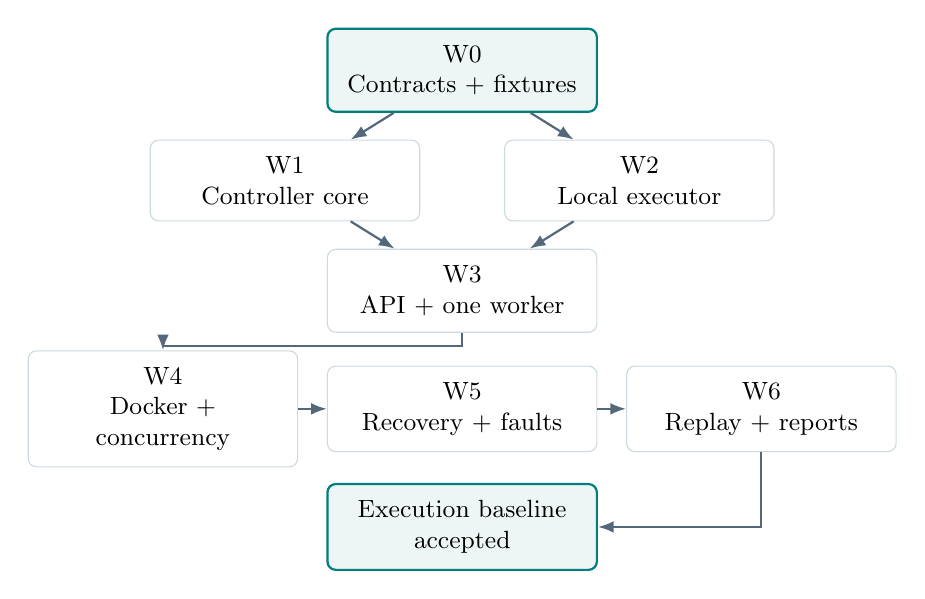
\begin{tikzpicture}
  \node[phase,active] (w0) at (0,0) {W0\\Contracts + fixtures};
  \node[phase] (w1) at (-2.25,-1.4) {W1\\Controller core};
  \node[phase] (w2) at (2.25,-1.4) {W2\\Local executor};
  \node[phase] (w3) at (0,-2.8) {W3\\API + one worker};
  \node[phase] (w4) at (-3.8,-4.3) {W4\\Docker + concurrency};
  \node[phase] (w5) at (0,-4.3) {W5\\Recovery + faults};
  \node[phase] (w6) at (3.8,-4.3) {W6\\Replay + reports};
  \node[phase,active] (gate) at (0,-5.8) {Execution baseline\\accepted};
  \draw[arrow] (w0) -- (w1);
  \draw[arrow] (w0) -- (w2);
  \draw[arrow] (w1) -- (w3);
  \draw[arrow] (w2) -- (w3);
  \draw[arrow] (w3.south) -- (0,-3.5) -- (-3.8,-3.5) -- (w4.north);
  \draw[arrow] (w4) -- (w5);
  \draw[arrow] (w5) -- (w6);
  \draw[arrow] (w6.south) -- (3.8,-5.8) -- (gate.east);
\end{tikzpicture}
\end{center}

\begin{tabularx}{\linewidth}{@{}P{0.36in}P{0.83in}YY@{}}
\toprule
 & \textbf{Depends on} & \textbf{Primary owner role} & \textbf{Gate evidence} \\
\midrule
W0 & Repo review & Interfaces / integration & Versioned contracts, lifecycle table and fixed fixtures. \\
W1 & W0 & Controller / storage & Transactional reservations and event reducer tests. \\
W2 & W0 & Worker / processes & Real process execution, logs, timeout and cancellation checks. \\
W3 & W1, W2 & Integration & Submit, execute, inspect and cancel through the API. \\
W4 & W3 & Runtime integration & Two Docker workers and concurrent placements without over-allocation. \\
W5 & W4 & Reliability / integration & Restart and message-loss scenarios with reconcilable outcomes. \\
W6 & W5 & Experiments / reporting & Repeatable workload replay and complete comparison reports. \\
\bottomrule
\end{tabularx}

\lead{Parallel work.} W1 and W2 share contracts, not mutable state. The replay manifest
and report schema can be designed during W3, while acceptance of experimental results
waits for W5. Roles describe ownership boundaries and can be combined by one developer.

\lead{Planning discipline.} Split each work package into reviewable changes with its gate
tests. Re-estimate remaining work after the first end-to-end W3 run. Early measurements
should determine polling intervals, launch overhead and test workload duration; this
document does not invent throughput targets or delivery dates.

\newpage
% PAGE 5
\pagetitle{FOUNDATION WORK}{Implement contracts, state and processes.}

\packet{W0}{Freeze the execution contracts}
\textbf{Deliver:} shared types, API/event versioning, lifecycle transitions, units
(CPU slots, MiB, seconds), validation rules and a small fixture workload. Define
submission idempotency, worker/session identity and attempt IDs before transport code.

Specify input availability and outputs: an immutable shared input mount for the local
prototype, per-attempt output directories, and bounded log retention or size limits.
Document that trusted jobs are expected to honor declared per-job resource requests.

\textbf{Gate:} fixtures cover a valid job, a request exceeding every configured worker's
total capacity (reject), a duplicate submission, a temporarily blocked queued job and
a job with no runtime estimate. State diagrams
explain cancellation before and after assignment. A configured worker inventory allows
validation even when a worker is temporarily offline.

\packet{W1}{Build the controller core and persistent store}
\textbf{Deliver:} a single-writer controller state machine, SQLite schema/migrations,
submission and event reducers, worker inventory, deterministic placement, and an
assignment-delivery outbox. Use explicit transactions for job state, attempt creation
and resource commitment. Rebuild authoritative state from persisted records on restart.

Expose a read-only scheduling snapshot and a picker interface. Preserve all queued jobs
in the snapshot: strict FIFO must be able to wait behind a temporarily blocked oldest job.
Store the policy version and selected action with each scheduling decision.

\textbf{Gate:} two competing assignments cannot exceed capacity; duplicate outcomes do
not free resources twice; stale session events cannot mutate a newer attempt; repeated
submissions resolve to the same job; restarting the controller preserves unresolved work.

\packet{W2}{Build a local executor library}
\textbf{Deliver:} process launch from an explicit argument list, configured environment
and working directory; per-attempt stdout/stderr files; exit status; monotonic timeout;
process-group cancellation with a grace period and forced termination when needed.
Drain output continuously or write directly to files so verbose jobs cannot deadlock on pipes.

Retain an attempt journal and unacknowledged events. Associate process evidence with the
attempt and execution session; a PID alone is insufficient after restart. Serialize
launch and cancellation per attempt. Persist cancellation markers and check them before
spawn so a delayed assignment cannot launch after cancellation is acknowledged.

\textbf{Gate:} real helper processes verify success, nonzero exit, launch failure,
large output, timeout, cancel-before-delivery, cancel-during-launch and parent exit with a
surviving child. Trusted jobs must not detach descendants from the managed process group.
Terminate remaining managed descendants and confirm the group stopped before any terminal
outcome releases capacity. Preserve the main exit result and record cleanup separately.

\callout{\textbf{Integration rule:} controller and executor changes can proceed in parallel
after W0. Keep their tests independent: the controller uses a fake worker transport;
the executor uses real local processes without requiring a controller or Docker.}

\newpage
% PAGE 6
\pagetitle{RUNTIME WORK}{Connect, package and recover.}

\packet{W3}{Add the API, worker agent and client}
\textbf{Deliver:} submit/status/cancel/log-access operations; worker registration and
polling; heartbeat/inventory exchange; assignment delivery; idempotent outcome ingestion.
The agent wraps W2. Workers retain outcome events until the controller commits and
acknowledges them. The client exposes job state and useful failure reasons.

Use an explicit command/event version and reject incompatible messages. Do not hold
database transactions open while waiting for network delivery. A timed-out delivery
keeps its existing attempt ID and reservation; it does not create a fresh attempt.

\textbf{Gate:} one controller and one worker run in separate processes. A client submits
a job, retrieves output and outcome, cancels a second job, and reconnects after a dropped
connection without duplicate launch. Reserved capacity is visible before RUNNING.

\packet{W4}{Add Docker workers and concurrent execution}
\textbf{Deliver:} a new custom-runner Dockerfile and Compose configuration with one
controller and two workers, persistent controller/worker state, inputs and output mounts,
health checks, and distinct worker identities. Existing Slurm files remain usable.

Configure worker-level CPU/memory limits and advertised schedulable capacities that
leave memory/CPU headroom for the worker agent.
Jobs run as child processes; Docker handles container limits, while the controller
accounts for per-job requests. Use a single serialized decision/commit path even when
multiple workers poll or report completions concurrently.

\textbf{Gate:} demonstrate execution on both workers, concurrent fitting jobs on one
worker, queueing when capacity is occupied, cancellation with later capacity reuse,
and a resource request that can fit only one configured worker. Confirm host capacity
is sufficient for the test; virtual quotas are not dedicated physical cores.

\packet{W5}{Verify recovery and lifecycle corner cases}
\textbf{Deliver:} reconciliation for controller restart, stale worker sessions, disconnects,
lost launch acknowledgments and duplicate reports. A disconnected worker is unavailable
for new assignments. New registration retains prior unresolved commitments. The current
reporting session may reconcile old execution-session attempts without modifying newer
attempts. Retry is explicit after the previous attempt is confirmed terminal.

Test crash points before/after reservation commit, delivery, launch journaling, process
creation and result acknowledgment. Reconciliation may require operator resolution in
the prototype when process evidence is insufficient. Do not turn uncertainty into an
unjustified success, failure, or second launch.

\textbf{Gate:} the fault matrix on the next page passes for supported cases. A controller
restart rebuilds the same unresolved allocations; terminal events survive worker/API
reconnection; cancellation during launch cannot be reported complete while work remains alive.

\newpage
% PAGE 7
\pagetitle{VERIFICATION AND EXPERIMENTS}{Make every claim observable.}
\label{testpage}
Tests should check externally meaningful outcomes and state invariants. Existing
simulator tests remain a regression gate when shared helpers are changed; no production
code should be rewritten merely to share a name or schema.

\begin{tabularx}{\linewidth}{@{}P{1.55in}YY@{}}
\toprule
\textbf{Scenario} & \textbf{Required assertion} & \textbf{Evidence} \\
\midrule
Concurrent dispatch & Commitments never exceed configured capacity. & Job/attempt state plus reservation ledger. \\
Repeated assignment & At most one actual launch per attempt in an uninterrupted session; an ambiguous crash gap triggers no new spawn. & Job-written start markers, process evidence and explicit UNKNOWN when needed. \\
Duplicate/out-of-order events & No double release or terminal-state regression. & Event IDs, transition history and final ledger. \\
Cancel / timeout & Confirm managed group termination; a delayed assignment cannot launch after cancellation. & Durable cancellation marker, child-process checks and timestamps. \\
Controller restart & Unresolved work and commitments survive. & Before/after inventory and persistent records. \\
Worker disconnect & No new assignments to that session; no automatic duplicate retry. & Health state and unchanged unresolved attempt ID. \\
No running jobs + Wait & Another decision is scheduled; no busy loop or deadlock. & Fake-clock event test and live timer test. \\
Strict FIFO head blocked & Later jobs do not bypass the head. & Ordered decisions and identical placement path. \\
\bottomrule
\end{tabularx}

\packet{W6}{Build replay and complete reports}
\textbf{Deliver:} an execution manifest containing arrivals, command templates, resources,
limits, seeds and input references. Generate single-worker jobs explicitly. Use sleep
jobs for lifecycle checks and CPU/memory helpers for execution experiments; a synthetic
runtime label is not itself an executable workload or a guaranteed wall-clock duration.

Capture controller-received submission time, reservation, launch/start evidence, finish,
exit status, worker/session, attempt ID, policy/configuration versions and resource
allocations. Report submission-to-completion response time, queue/start delay,
throughput, tail waiting and allocation utilization. Label allocation utilization
separately from measured CPU/memory usage.

\textbf{Comparison protocol:} reuse the same controller, worker code, placement, failure
rules and measurements; change only the picker. Replay identical manifests from
equivalent clean starting conditions. Alternate policy run order and repeat runs to
expose shared-host variation. Record measured submission timing as well as intended arrivals.

\textbf{Gate:} reports account for every submitted job, including failures and unfinished
work. Complete successful workloads support response-time comparisons. Incomplete or
failed runs remain clearly marked; averaging only successful jobs must not be presented
as an improvement. Check that admission delay and launch latency remain in response time.

\callout{\textbf{Baseline naming:} strict FIFO waits if the oldest queued job cannot fit.
Selecting the oldest job that fits is a separate baseline. Both can use the same system,
but their behavior and names must not be conflated.}

\newpage
% PAGE 8
\pagetitle{FUTURE PICKER HANDOFF}{Prepare the interface without building RL now.}
The execution project ends with a dependable policy-independent runner. A subsequent
workstream can implement a sequential simulator and RL picker against the same contract.
The model controls job selection and waiting; placement, reservations, launch, cancellation
and reconciliation remain execution-system responsibilities.

\begin{center}
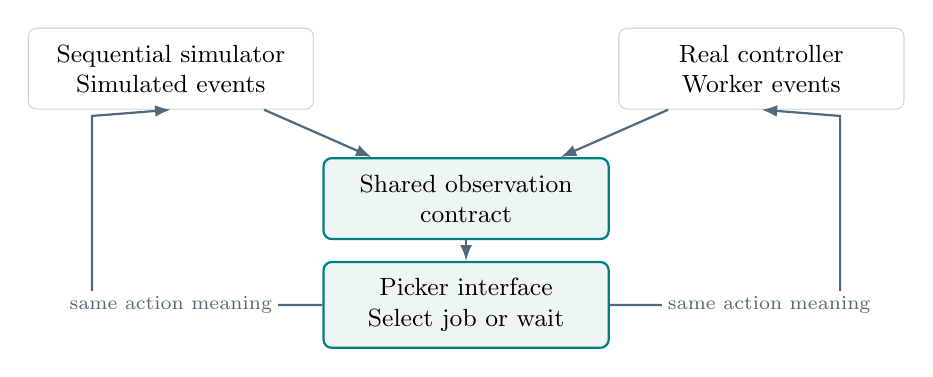
\begin{tikzpicture}
  \node[box,text width=3.2cm] (sim) at (0,0) {Sequential simulator\\Simulated events};
  \node[box,text width=3.2cm] (live) at (7.5,0) {Real controller\\Worker events};
  \node[active,text width=3.2cm] (obs) at (3.75,-1.65) {Shared observation\\contract};
  \node[active,text width=3.2cm] (policy) at (3.75,-3.0) {Picker interface\\Select job or wait};
  \draw[arrow] (sim) -- (obs);
  \draw[arrow] (live) -- (obs);
  \draw[arrow] (obs) -- (policy);
  \draw[arrow] (policy.west) -- (-1,-3.0) -- (-1,-0.6) -- (sim.south);
  \draw[arrow] (policy.east) -- (8.5,-3.0) -- (8.5,-0.6) -- (live.south);
  \node[flowlabel] at (0,-3.0) {same action meaning};
  \node[flowlabel] at (7.6,-3.0) {same action meaning};
\end{tikzpicture}
\end{center}

\lead{Required compatibility.} Expose all queued requests with feasibility information,
including committed-but-not-started allocations. Use stable job IDs and a snapshot
version. A stale policy response is revalidated or recomputed before commitment.
Do not expose actual runtime, exact remaining duration, or future arrivals to the policy.

\lead{Waiting and progress.} Wait ends at the next arrival, completion, worker-state
change, or positive control tick. Any operational limit on voluntary idling must be
configured, observed by the policy, shared across simulation and execution, and logged.
Never infer that waiting is invalid from hidden knowledge that a trace has no future jobs.

\lead{Simulation changes later.} Existing \code{simulate()} runs a complete fixed-weight
trace and rejects some idle states that a waiting policy needs. The new environment must
expose decisions and account for launch delay and committed resources. Preserve the legacy
replay path and its regression tests. Match logical semantics, not exact wall-clock timestamps.

\lead{Research distinction.} DeepRM selects a job for earliest feasible future placement
in a pooled resource calendar. Our proposed first picker selects a job for dispatch now
on an individual worker. Training must reflect this adaptation. The current Gaussian
weight-bandit network and full-trace features are not a drop-in sequential controller.

\lead{Metrics are ready for future rewards.} For complete episodes, the integral of
arrived, unfinished jobs measures total response time:
\[
  \int N_{\mathrm{unfinished}}(t)\,dt
  = \sum_j (t_{\mathrm{finish},j}-t_{\mathrm{submit},j}).
\]
Queued, reserved and running jobs all count. Dividing by the number of jobs gives mean
response time. Record failures and incomplete work explicitly rather than allowing them
to disappear from a future reward or comparison.

\newpage
% PAGE 9
\pagetitle{REVIEW AND REPOSITORY MAP}{Close the design gaps before implementation.}
\label{reviewpage}
\textbf{Review status:} two independent agent reviews assessed architecture/lifecycle and
implementation/test design. Both found the overall architecture and delivery order sound.
The corrections below are incorporated. Review assessed the plan only; no runtime or
system tests were implemented as part of this document.

\begin{tabularx}{\linewidth}{@{}P{1.55in}Y@{}}
\toprule
\textbf{Issue examined} & \textbf{Disposition in this plan} \\
\midrule
Session reconciliation & Separate reporting from execution sessions; reconcile old attempts while preserving unresolved commitments and protecting newer attempts. \\
Delayed assignment after cancel & Persist cancellation markers before acknowledgment; serialize launch/cancel and check the marker before spawn. \\
Children outlive parent & Trusted jobs stay in the managed process group. Clean up remaining descendants before terminal reporting and capacity release. \\
Weak duplicate-launch test & Count actual starts using job-written markers and process evidence, rather than counting acknowledgments. \\
Acceptance allows uncertainty & Normal fixtures must reach their expected terminal outcomes with no UNKNOWN. Uncertainty is limited to explicit ambiguous fault tests. \\
Impossible versus blocked & Reject requests exceeding all configured workers; queue temporarily blocked jobs. Strict FIFO preserves head-of-queue blocking. \\
Milestone ambiguity & W4 is the first two-worker demonstration; W6 is the accepted baseline with recovery evidence and complete reports. \\
\bottomrule
\end{tabularx}

\lead{Proposed module boundaries.} Names below describe new work, not existing files:

\begin{tabularx}{\linewidth}{@{}P{2.65in}Y@{}}
\toprule
\textbf{Proposed location} & \textbf{Responsibility} \\
\midrule
\code{execution/models.py} & Job, worker, attempt, event and observation contracts. \\
\code{execution/store.py}, \code{controller.py} & Durable transitions, reservations, decisions and reconciliation. \\
\code{execution/executor.py}, \code{worker.py} & Local process lifecycle, polling and event delivery. \\
\code{execution/api.py}, \code{cli.py} & Controller transport and user operations. \\
\code{execution/replay.py}, \code{reporting.py} & Workload manifests, replay and complete reports. \\
\code{compose.execution.yaml} & Separate controller/worker deployment for this system. \\
\bottomrule
\end{tabularx}

\lead{Reuse carefully.} Resource compatibility and placement ideas live in
\code{src/slurm\_aware/simulator.py}; trace generation is in \code{workloads.py}.
The existing \code{rl/} package is the weight-bandit baseline. Extract shared helpers only
when tests demonstrate unchanged behavior. Existing local changes, legacy runtime-model
experiments, Slurm Docker files and PDFs are not cleanup targets for this work.

\lead{First implementation batch.} W0 contracts and fixtures, followed by independent
W1 controller-state and W2 executor changes. Integrate only after their gates pass.
The first demonstration uses the same system with a simple picker; RL is a later swap.

\newpage
% PAGE 10
\pagetitle{ACCEPTANCE AND REFERENCES}{Define what a finished first system means.}

\lead{Execution baseline acceptance.} A fresh checkout plus documented dependencies can
start the new Compose setup. Submit a fixed mixed workload, inspect jobs and workers,
retrieve outputs, cancel a running job and observe correct capacity reuse. Run the
same workload again from clean state and produce another complete report.

\begin{itemize}
\item The normal fixture workload reaches every expected terminal outcome (including
intentional failures, timeouts and cancellations), with no unresolved attempts.
\item UNKNOWN is an expected outcome only for explicitly injected ambiguous faults.
Every job and attempt remains traceable to its outcome or recorded uncertainty.
\item Resource commitments include delivery/startup, remain within configured capacity,
and are released once after definitive evidence.
\item Restart and delivery fault tests demonstrate supported recovery behavior without
claiming that every arbitrary crash can be resolved automatically.
\item Reports identify the workload, configuration, policy version, environment and all outcomes.
\item FIFO and any future picker share the execution, placement, timeout and reporting paths.
\end{itemize}

\lead{Decisions to record in W0.} Confirm Python-first implementation; select worker
capacities and input/output mounts for the available host; choose heartbeat and decision
timer defaults through measurement; specify the trusted-job resource contract and the
procedure for unresolved attempts. These are configuration/design decisions, not reasons
to begin with a larger distributed platform.

\lead{Evidence used.} Repository inspection at HEAD \code{06a6416}, including the dirty
working tree, informed the reuse boundaries. The existing simulator and documentation
provide context; this plan does not claim that their tests validate the new runtime.

\begin{enumerate}[label={[\arabic*]},leftmargin=22pt,itemsep=7pt]
\item \textbf{Current simulator:} \code{src/slurm\_aware/simulator.py}. The live-runtime
separation follows from \code{Job} requiring runtime and rejecting runtime above its limit;
\code{simulate()} currently controls a complete replay.
\item \textbf{Current workloads and learner:} \code{src/slurm\_aware/workloads.py} and
\code{src/slurm\_aware/rl/}. Generator outputs include multi-node jobs; current training
uses one Gaussian weight action per trace, with hindsight-derived features.
\item \textbf{DeepRM:} H. Mao, M. Alizadeh, I. Menache and S. Kandula,
\emph{Resource Management with Deep Reinforcement Learning}, HotNets 2016.
Local source: \code{deeprm\_hotnets16.pdf}. Sections 3 and 5 inform the action semantics
and the limitations of pooled resources and known durations.
\item \textbf{Python subprocess execution:}
\href{https://docs.python.org/3.11/library/asyncio-subprocess.html}{Python 3.11 asyncio subprocess documentation}.
Supports the proposed asynchronous worker executor.
\item \textbf{Docker networking:}
\href{https://docs.docker.com/compose/how-tos/networking/}{Networking in Compose}.
Supports the local controller/worker service topology.
\item \textbf{Docker limits:}
\href{https://docs.docker.com/engine/containers/resource_constraints/}{Resource constraints}.
Supports worker-container CPU/memory limits; it does not make reservations into per-job limits.
\end{enumerate}

\lead{Document reproduction.} The accompanying \code{scheduler-work-plan.tex} contains
the text and TikZ diagrams. Compile with:
\begin{quote}\ttfamily\small
tectonic --untrusted --keep-logs scheduler-work-plan.tex
\end{quote}
This PDF is a reviewed work plan. Creating it did not implement the controller, launch
workers, alter application code, install RL dependencies, or start containers.

\end{document}
